\documentclass[]{article}
\usepackage{graphicx}
\usepackage{wrapfig}
\usepackage{gensymb}
\usepackage{float}
\usepackage{hyperref}
\usepackage[slovene]{babel}
\usepackage{amsmath}
\usepackage[utf8x]{inputenc}
\usepackage{subcaption}
\usepackage[left=3.5cm,right=3.5cm]{geometry}
\usepackage{amssymb}
\usepackage{mathtools}
\usepackage{amsmath}
\hypersetup{
	colorlinks=true,
	linkcolor=blue,
	filecolor=magenta,      
	urlcolor=cyan,
}
%\usepackage[compact]{titlesec}         % you need this package
%\AtBeginDocument{%                     % this will reduce spaces between parts (above and below) %of texts within a (sub)section to 0pt, for example - like between an 'eqnarray' and text
%	\setlength\abovedisplayskip{10pt}
%	\setlength\belowdisplayskip{10pt}}

%za newline v tabeli
\usepackage{pbox}

\usepackage{longtable}


\begin{document}

\title{Samopodobnost standardne preslikave Chririkovega}

\author{Alja\v z  Pav\v sek}

\date{18. januar 2020}

\maketitle

\section{Navodilo naloge}
Ilustriraj hierarhijo faznega prostora v "sibko kaoti"cni standardni preslikavi. Izberi zaporedje pove"cav sekundarnih otokov regularnega gibanja (Poincar\'e-Birkhoffovih resonanc) pri primernem parametru, k $\sim$ 1.
Napravi npr. zaporedje kakih 5-6 sli"cic, kjer je vsaka primerna pove"cava detajla prej"snje. Komentiraj samopodobnost v statisti"cnem smislu.

\section{Uvod}
Preden se lotimo konstrukcije problema in analize rezultatov, je pametno ponoviti nekaj pojmov, ki so neposredno povezani z našim problemom.


\subsection{Brcan rotator in standardna preslikava}
Standardna preslikava Chirikova, ki je eden od najbolj temeljito preu"cevanih dinami"cnih sistemov, temelji na realnem fizikalnem sistemu tako imenovanega 'brcanega rotatorja'. Imamo palico z vztrajnostnim momentom $\bar{I}$, ki je vpeta na enem koncu in dopu"s"ca rotacijo okoli ene osi, pri "cemer zanemarimo trenje (slika \ref{slika 1}). Palico v periodi"cnih sunkih brcamo v navpi"cni smeri (glede na sliko \ref{slika 1}).
\begin{figure}[!htb]
	\begin{center}
		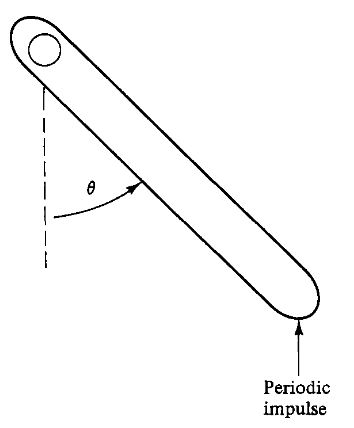
\includegraphics[width = 7cm]{kicked_rotator}
		\caption{Brcani rotator. Vir: \cite{1}}
		\label{slika 1}
	\end{center}
\end{figure}
"Casovno odvisni Hamiltonijan takega sistema in njemu pripadajo"ce dinami"cne ena"cbe so
\begin{equation}\label{1}
\begin{aligned}
\text{H}(p,\theta,t)=&\frac{p^2}{2\bar{I}}+k\cos\theta\sum_n\delta(t-n\tau)\\
\frac{dp}{dt}=k&sin\theta\sum_n\delta(t-n\tau)\\
&\frac{d\theta}{dt}=\frac{p}{\bar{I}}.
\end{aligned}
\end{equation}
Kot $p_n$ in $\theta_n$ ozna"cimo vrednosti $p$ in $\theta$ pri "casih $t=n\tau+0^+$. "Ce zgornji dinami"cni ena"cbi integriramo preko enega periodi"cnega "casovnega intervala (do $t=(n+1)\tau+0^+$), dobimo diskretizirano "casovno evolucijo
\begin{equation}\label{2}
\begin{aligned}
p_{n+1}&=p_n+ksin\theta_{n+1}\ \mod{2\pi}\\
&\theta_{n+1}=\theta_n+p_n\ \mod{2\pi}.
\end{aligned}
\end{equation}
Vzeli smo $\tau/\bar{I}=1$ in upo"stevali periodi"cnost $\theta$. Prav tako smo upo"stevali periodi"cnost v $p$, kar se izka"ze za eno glavnih lastnosti standardne preslikave. Omenimo "se, da je preslikava simplekti"cna, torej ohranja diferencial 'simplekit"cnega obmo"cja' \cite{1}. Prav tako poudarimo, da vsi Hamiltonski sistemi ohranjajo 2N dimenzionalen volumen faznega prostora.

\subsection{KAM teorem}
N-dimenzionalni Hamiltonski sistemi $\text{H}(\boldsymbol{p},\boldsymbol{q})$, ki niso eksplicitno odvisni od "casa, so integrabilni, "ce jim lahko najdem N neodvisnih konstant gibanja. Za tak sistem obstaja kanoni"cna transformacija v tako imenovane 'action-angle' spremenljivke $(\boldsymbol{I},\boldsymbol{\theta})$. V brezdimenzijski obliki te spremenljivke te"cejo med $0$ in $2\pi$. Za Hamiltonijan v taki obliki je zna"cilno, da ni ve"c odvisen od prostorske koordinate $\boldsymbol{\theta}$. To nam da
\begin{equation}
\begin{aligned}
&-\frac{d\boldsymbol{I}}{dt}=\frac{\partial \text{H}(\boldsymbol{I})}{\partial \boldsymbol{q}}=0\\
&\frac{d \boldsymbol{\theta}}{dt}=\frac{\partial \text{H}(\boldsymbol{I})}{\partial \boldsymbol{\theta}}\equiv\boldsymbol{\omega}(\boldsymbol{I})\\
&\qquad\qquad\text{oz.}\\
&\boldsymbol{\theta}(t)=\boldsymbol{\theta}(0)+\boldsymbol{\omega}(\boldsymbol{I})t.
\end{aligned}
\end{equation}
Komponente $\boldsymbol{\omega}$ so frekvence, s katerimi to"cke faznega prostora z neko energijo kro"zijo po irudecibilnih zankah N dimenzionalnega torusa (slika \ref{slika 2}).
\begin{figure}[!htb]
	\begin{center}
		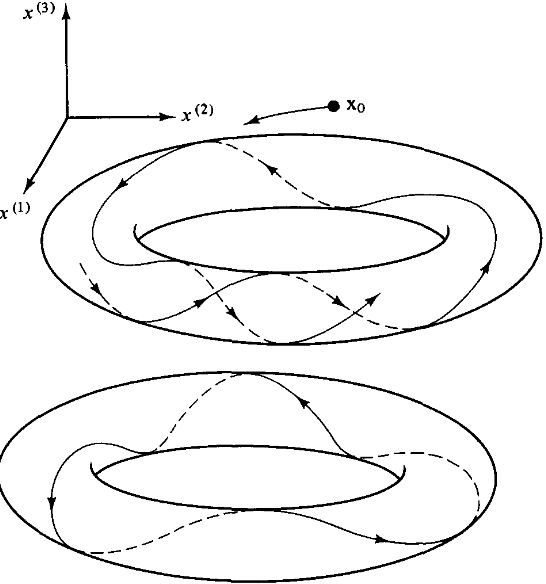
\includegraphics[width = 7cm]{torus}
		\caption{2D torus v 3D. Kvaziperiodi"cna (zgoraj) in periodi"cna (spodaj) orbita Vir: \cite{1}}
		\label{slika 2}
	\end{center}
\end{figure}
\noindent "Ce so razmerja posameznih komponent $\boldsymbol{\omega}$ enaka nekim razmerjem celih "stevil $m_i/m_j$, $1\leq i,j\leq N$, se orbita po $n$ obhodih zaklju"ci sama vase, "ce pa takih "stevil ni mogo"ce najti, trajektorija enakomerno zapolni cel torus. Za tako kvaziperiodi"cno orbito karekterizirano z $\boldsymbol{\omega}$ torej ne obstaja vektor $\boldsymbol{m}$ ($m_i\in\mathbb{Z}-\{0\}$), da bi veljalo
\begin{equation}
\boldsymbol{\omega}\cdot\boldsymbol{m}=0.
\end{equation}
KAM teorem nam podaja pogoj, glede na katerega bomo vedeli, "ce bo po neki majhni perturbaciji originalnega integrabilnega Hamiltonijana $\text{H}_0(\boldsymbol{I})$ ta ostal integrabilen. Ho"cemo torej najti taka nova $\boldsymbol{I}'$ in $\boldsymbol{\theta}'$, da bomo perturbiran Hamiltonijan
\begin{equation}\label{5}
\text{H}(\boldsymbol{I},\boldsymbol{\theta})=\text{H}_0(\boldsymbol{I})+\epsilon\text{H}_1(\boldsymbol{I},\boldsymbol{\theta})
\end{equation}
lahko zapisali kot H$(\boldsymbol{I}')$. Brez dokazovnja o pravkar opisanem problemu povejmo le to, da je klju"cnega pomena za obstoj orbite po perturbaciji prav $\boldsymbol{\omega}\cdot\boldsymbol{m}\neq 0$. Za take N-dimenzionalne toruse pravimo, do so neresonantni.\newline

\subsection{Poincar\'e-Birkhoffov teorem}
Kaj pa se zgodi z resonantnimi torusi, za katere velja $\boldsymbol{\omega}\cdot\boldsymbol{m}=0$ in na kateirih imamo prave periodi"cne orbite? Kot smo "ze omenili, ti torusi ne pre"zivijo perturbacije.\newline
Preu"cimo zadevo na primeru dinami"cnega sistema z dvema prostostnima stopnjama (N=2), katerega fazni prostor lahko opi"semo z 'angle-action' koordinatami ($\theta_1$, $\theta_2$, $I_1$, $I_2$). "Ce izvedemo Poincar\'ejevo redukcijo in fiksiramo npr. $\theta_2$, dobimo diskretno preslikavo na ravnino (slika \ref{slika 3}). Preseki torusov in ravnine so sklenjene zanke, ki jih lahko brez izgube splo"snosti obravnavamo kot koncentri"cne kroge.
\begin{figure}[!htb]
	\begin{center}
		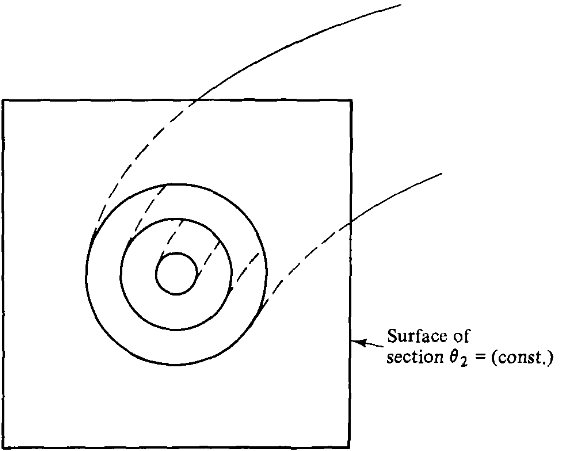
\includegraphics[width = 7cm]{crosssection}
		\caption{Levo: Presek dvodimezionalnega torusa z ravnino $\theta_2=konst.$ Desno: Periodi"cna orbita na resonantnem torusu. Vir: \cite{1}}
		\label{slika 3}
	\end{center}
\end{figure}
\noindent To"cke v tem prostoru lahko popolnoma opi"semo s polarnimi koordinatami; $\phi\equiv\theta_1$, ki je periodi"cna na $2\pi$ in $I_1$, ki je proporcionalen radiju kro"znic $r$. Dobimo diskretno preslikavo $(r_{n+1},\phi_{n+1})=\boldsymbol{M}_0(r_{n},\phi_{n})$:
\begin{equation}
\begin{aligned}
&r_{n+1}=r_n\\
&\phi_{n+1}=\phi_{n}+2\pi R(r_n) \mod 2\pi,
\end{aligned}
\end{equation}
kjer smo z rotacijskim "stevilom $R(r_n)$ ozna"cili razmerje frekvenc $\omega_1/\omega_2$ ($\boldsymbol{\omega_0}=(\omega_1,\omega_2)=(\partial\text{H}_0/\partial I_1,\partial\text{H}_0/\partial I_2)$), ki je za resonanten torus enako razmerju dveh celih, neni"celnih "stevil $m/n$. O"citno je, da bo trajektorija po $n$ obhodih celega torusa ($\phi_2$ od $0$ do $2\pi$) prispela nazaj v prvotno pozicijo (slika \ref{slika 2} spodaj), n-krat aplicirana preslikava $(\boldsymbol{M}_0)^n\equiv\boldsymbol{M}_0^n$ torej to"cke iz resonantnega torusa karakteriziranega z $\omega_1/\omega_2$, prevede nazaj vase
\begin{equation}
\boldsymbol{M}_0^n(r_{n+1},\phi_{n+1})=[r_{n},\ \phi_{n}+2\pi m \mod 2\pi]=(r_{n},\phi_{n}).
\end{equation}
\begin{figure}[!htb]
	\begin{center}
		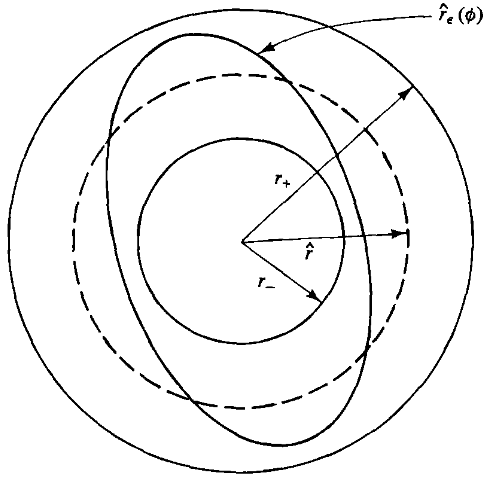
\includegraphics[width = 4.7cm]{41}
		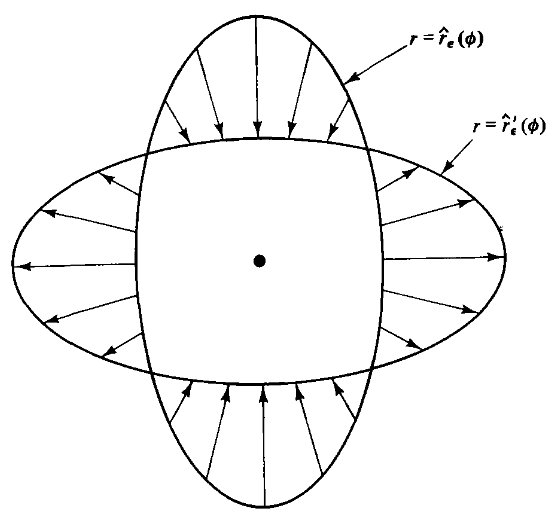
\includegraphics[width = 4.7cm]{42}
		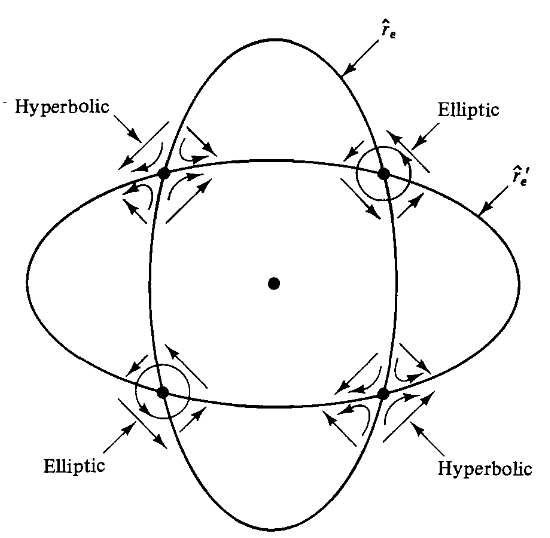
\includegraphics[width = 4.7cm]{43}
		\caption{Preslikava $\boldsymbol{M}_\epsilon^n$. Nevtralen krog, (na katerem ni zasuka), se po perturbaciji deformira v $r_\epsilon(\phi)$ (levo), ki ga preslikava $\boldsymbol{M}_\epsilon^n$ slika v $r_\epsilon(\phi)$ (sredina), kar rezultira v kreaciji sodega "stevila elipti"cnih in hiperboli"cnih to"ck. Vir: \cite{1}}
		\label{slika 4}
	\end{center}
\end{figure}
Predpostavimo, da je $\boldsymbol{M}_0^n$ v okolici resonantnega 'KAM' kroga neni"celna v prvem odvodu. To pomeni, da se "ze pri majhni spremembi $r$ to"cke na krogu z manj"sim $r^-<r$ po preslikavi $\boldsymbol{M}_0^n$ zasukajo v npr. pozitivni smeri. Prav tako se to"cke pri malo ve"cjem $r^+>r$ po preslikavi $\boldsymbol{M}_0^n$ zasukajo v negativni smeri. Na preu"cevanem resonantem torusu s periodo n, kot "ze omenjeno po $\boldsymbol{M}_0^n$ ni spremembe v $\phi$.\newline
Po majhni perturbaciji Hamiltonijana (\ref{5}) dobimo  $\boldsymbol{M}_\epsilon$:
\begin{equation}
\boldsymbol{M}_\epsilon(r_{n+1},\phi_{n+1})=[r_{n}+\epsilon g(r_n,\phi_{n}),\ \phi_{n}+2\pi R(r_n) + \epsilon h(r_n,\phi_{n}) \mod 2\pi]=(r_{n},\phi_{n}).
\end{equation}
Prav tako kot je v primeru pred perturbacijo med $r^+$ in $r^-$ obstajala kro"znica, na kateri se po preslikavi $\boldsymbol{M}_0^n$ to"cke niso zasukale, mora po perturbaciji obstajati zanka $r_\epsilon(\phi)$ (slika \ref{slika 4} levo), na kateri se to"cke slikajo v  $r_\epsilon'(\phi)$ kve"cjemu v radialni smeri (slika \ref{slika 4} sredina). Ker se volumen preslikave ohranja, se krivulji $r_\epsilon(\phi)$ in $r_\epsilon'(\phi)$ sekata v sodem "stevilu to"ck (verjetnost, da se krivulji tangentno stakneta, je glede na scenarij, ko se krivulji sekata, prakti"cno 0). "Ce preu"cimo tok to"ck v reduciranem faznem prostoru pri taki preslikavi, ugotovimo, da z majhno perturbacijo H$_0$ resonantne KAM krivulje s periodo n razpadejo na sodo "stevilo fiksnih to"ck preslikave $\boldsymbol{M}_\epsilon^n$, polovica katerih so elipti"cne in polovica hiperboli"cne to"cke (slika \ref{slika 4} desno). \newline
Nadaljnje opazimo, da ker so prese"ci"s"ca $r_\epsilon(\phi)$ in $r_\epsilon'(\phi)$ fiksne to"cke  preslikave $\boldsymbol{M}_\epsilon^n$, mora po perturbaciji iz resonantnega torusa z rotacijskim "stevilom $m/n$ nastati n (ali ve"ckratnik n) elipti"cnih in prav tako "stevilo hiperboli"cnih to"ck (slika \ref{slika 5}).
\begin{figure}[!htb]
	\begin{center}
		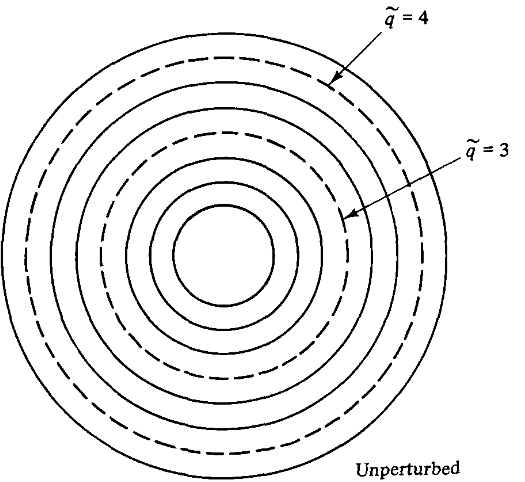
\includegraphics[width = 6cm]{6}
		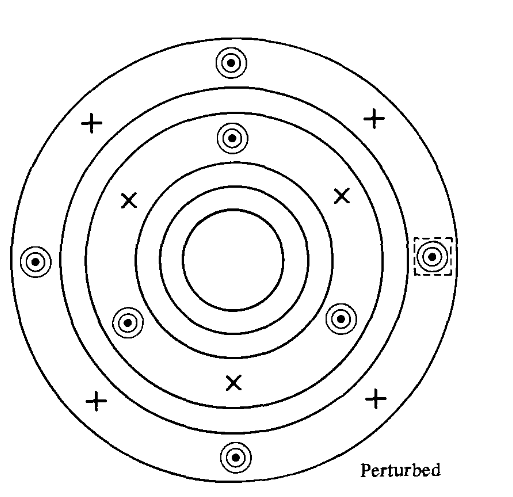
\includegraphics[width = 6cm]{7}
		\caption{Iz resonantenga torusa, na katerem so orbite periode $\tilde{q}$ nastane $\alpha\tilde{q}$ hiperboli"cnih in $\alpha\tilde{q}$ elipti"cnih to"ck, $\alpha$ je neko neznano naravno "stevilo. Okoli novo nastalih elipti"cnih to"ck se pojavijo nove $q'$ periodi"cne orbite (razli"cni $q'$), ki prav tako razpadejo. Zgodba se ponavlja v neskon"cnost. Vir: \cite{1}}
		\label{slika 5}
	\end{center}
\end{figure}
Okoli novih elipti"cnih to"ck imamo prav tako neresonantne in resonantne KAM krivulje z novimi rotacijskimi "stevili. Slednje prav tako po perturbaciji razpadejo na nove verige elipti"cnih otokov. Dobljena slika je sebi-podobna v fraktalnem smislu - na vseh velikostnih skalah lahko najdemo podobne strukture.
Omenimo lahko "se, da po zadostni perturbaciji za"cetnega Hamiltonijana pri"cnejo razpadati tudi neresonantni torusi. Stopnja perturbacije, ki je potrebna, da neresonantni torusi razpadejo, je neposredno povezana s 'stopnjo iracionalnosti' rotacijskega "stevila $R$ (kako hitro aproskimacija $R_n$ konvergira k pravi vrednosti, ko v reprezentaciji $R_n$ z veri"znim ulomkom zaporedno dodajamo "clene $a_i$)
\begin{equation}\label{9}
R_n=[a_1,a_2,...,a_n,0,0,0,...]\qquad R=\lim\limits_{n\to\infty}R_n.
\end{equation}

\section{Samopodobnost standardne preslikave}

\subsection{Konstrukcija kode}
Izberemo mre"zo $n\times n$ za"cetnih pogojev znotraj obmo"cja $\Sigma=[x-10^{-m}\pi,x+10^{-m}\pi]\times[p-10^{-m}\pi,p+10^{-m}\pi]$ za $m$-kratno pove"cavo. Za"cnemo izvajati iteracijo - propagiramo $n^2$ to"ck po en "casovni korak naprej. Ko se na $\Sigma$ nabere "zeljeno "stevilo to"ck ($\mathcal{O}(10^5)$), iteracijo ustavimo in nari"semo to"cke, ki izvirajo iz enakega za"cetnega pogoja z enako barvo.

\begin{figure}[!htb]
	\begin{center}
		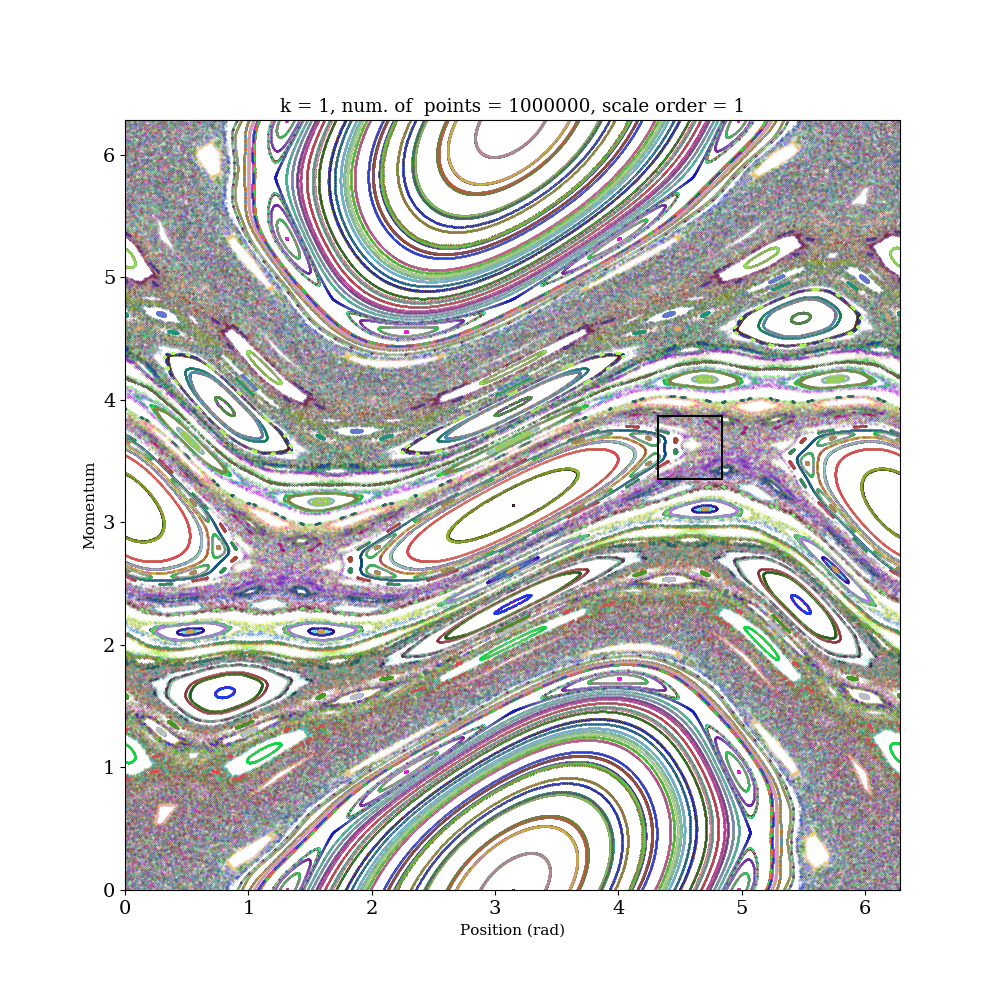
\includegraphics[width = 11cm]{stdmap1}
		\caption{Standardna preslikava pri k=1. Vir: \cite{1}}
		\label{slika 6}
	\end{center}
\end{figure}
\begin{figure}[!htb]
	\begin{center}
		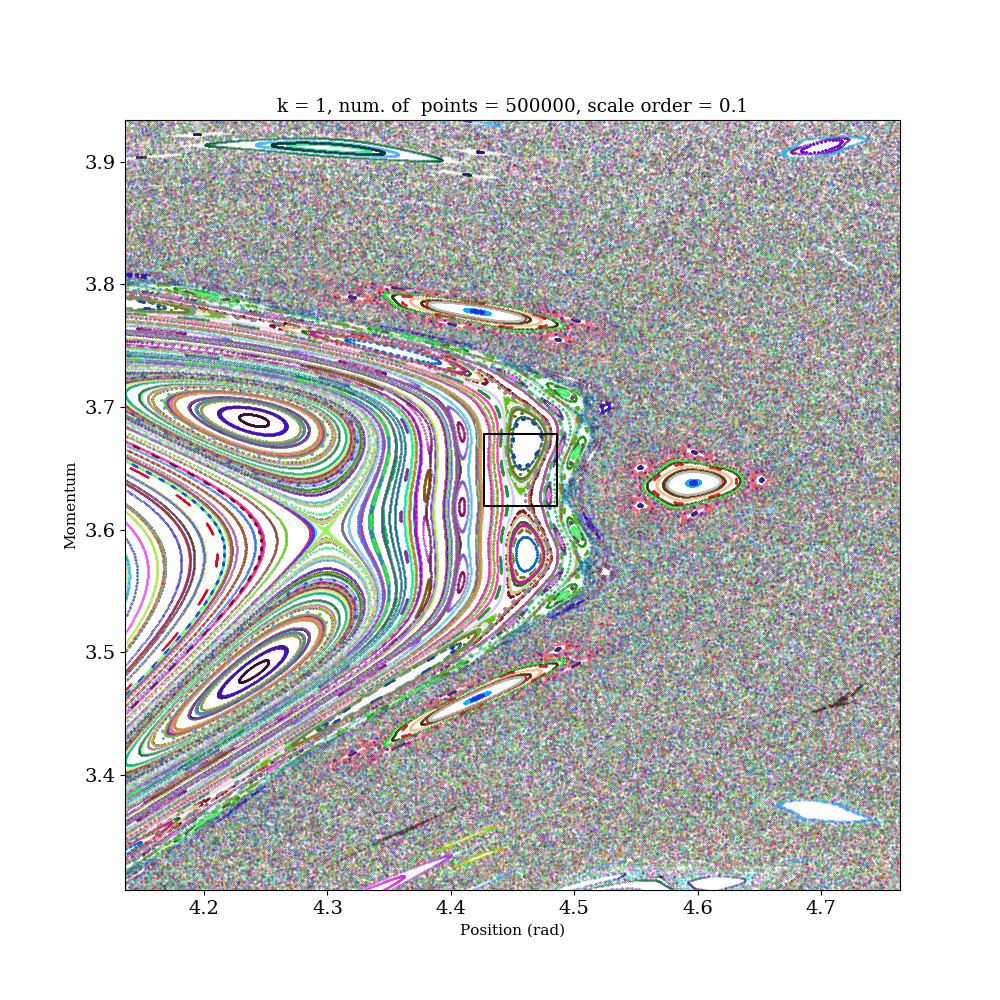
\includegraphics[width = 11cm]{stdmap2}
		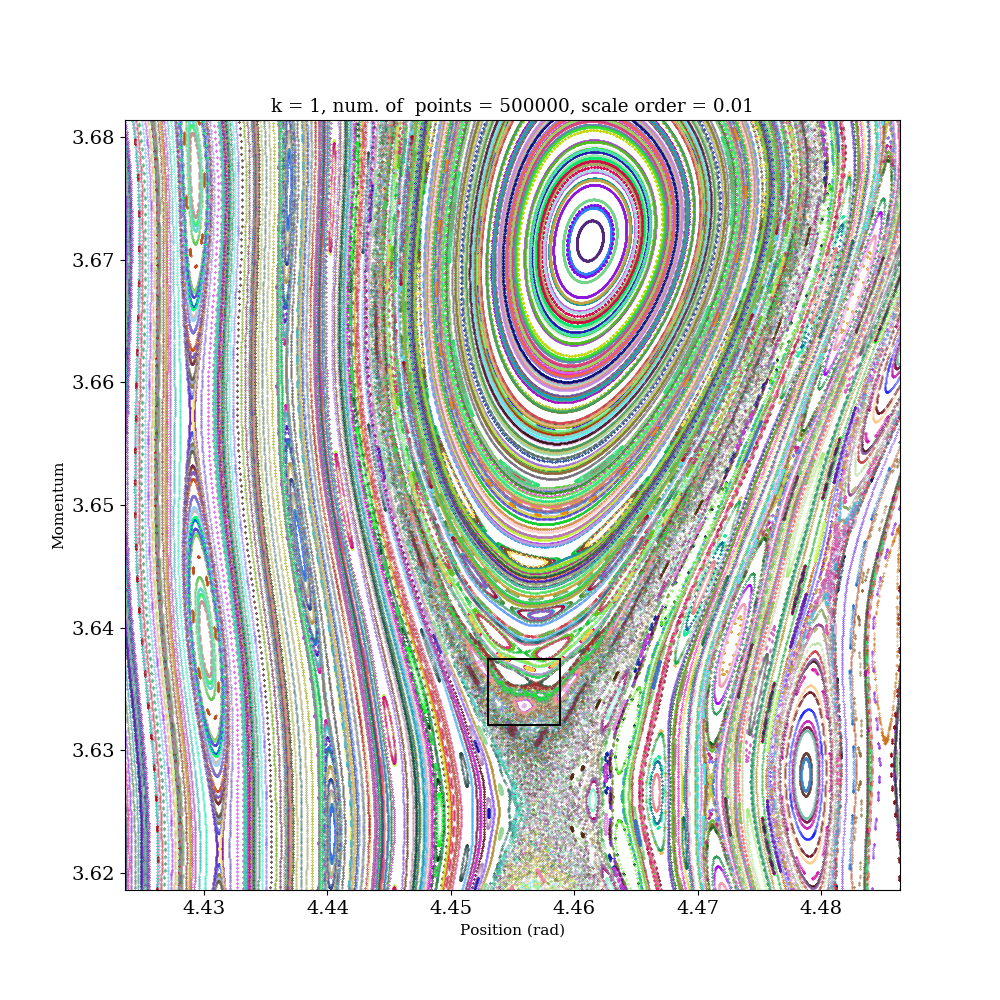
\includegraphics[width = 11cm]{stdmap3}
		\caption{Standardna preslikava pri k=1, enkratna (m=1) in dvokratna (m=2) pove"cava. Vir: \cite{1}}
		\label{slika 7}
	\end{center}
\end{figure}
\begin{figure}[!htb]
	\begin{center}
		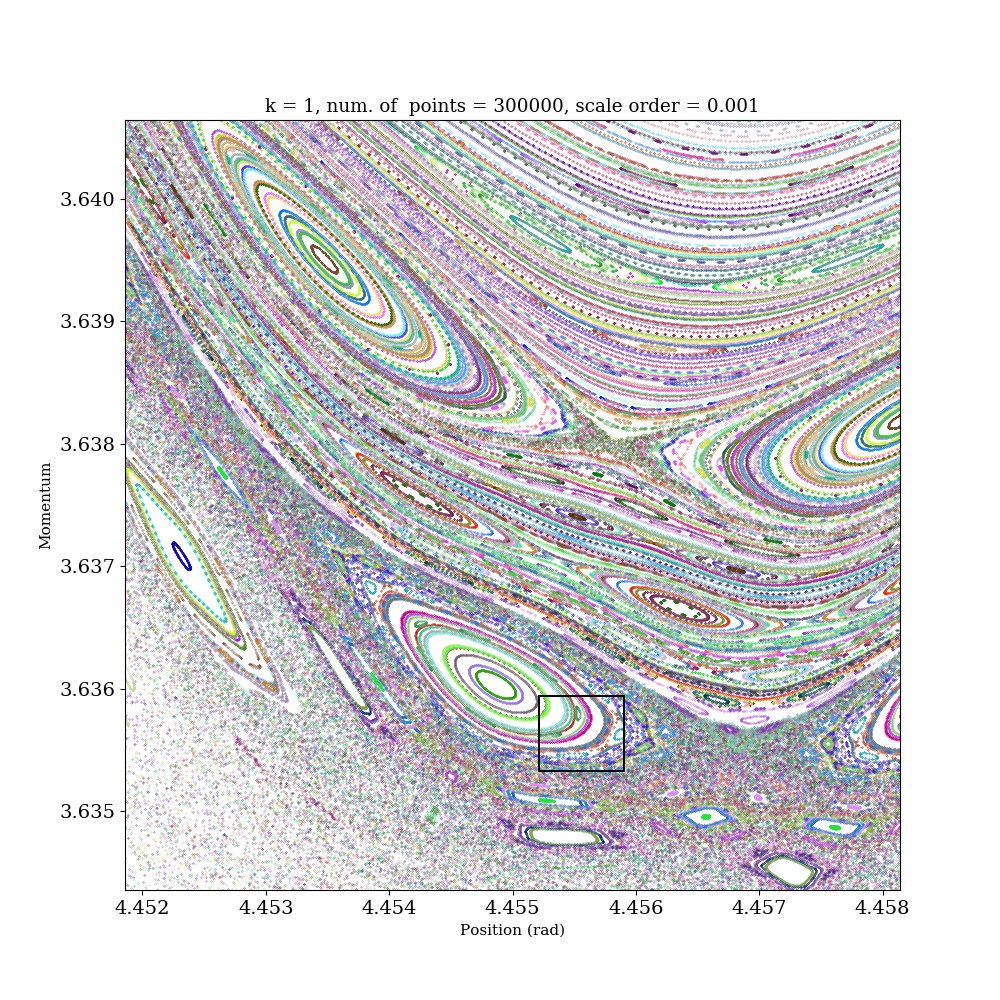
\includegraphics[width = 11cm]{stdmap4}
		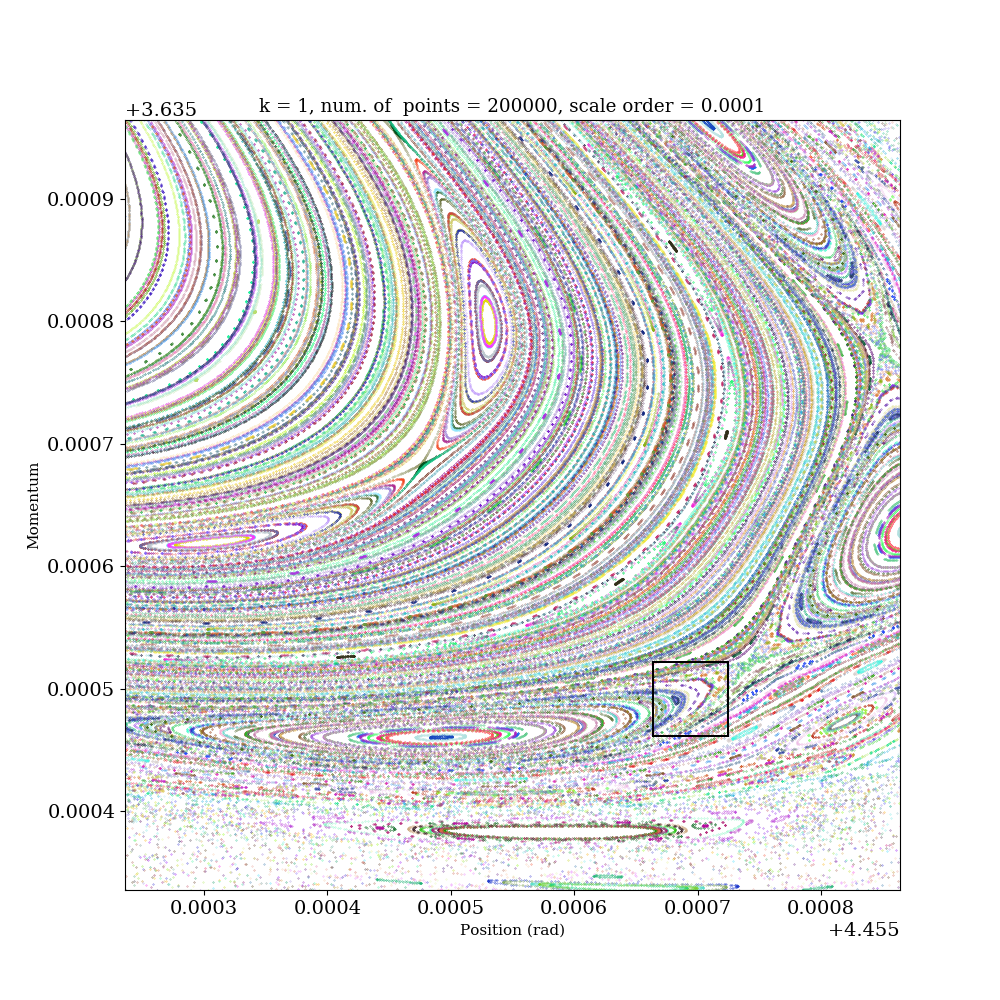
\includegraphics[width = 11cm]{stdmap5}
		\caption{Standardna preslikava pri k=1, enkratna (m=3) in dvokratna (m=4) pove"cava. Vir: \cite{1}}
		\label{slika 8}
	\end{center}
\end{figure}
\begin{figure}[!htb]
	\begin{center}
		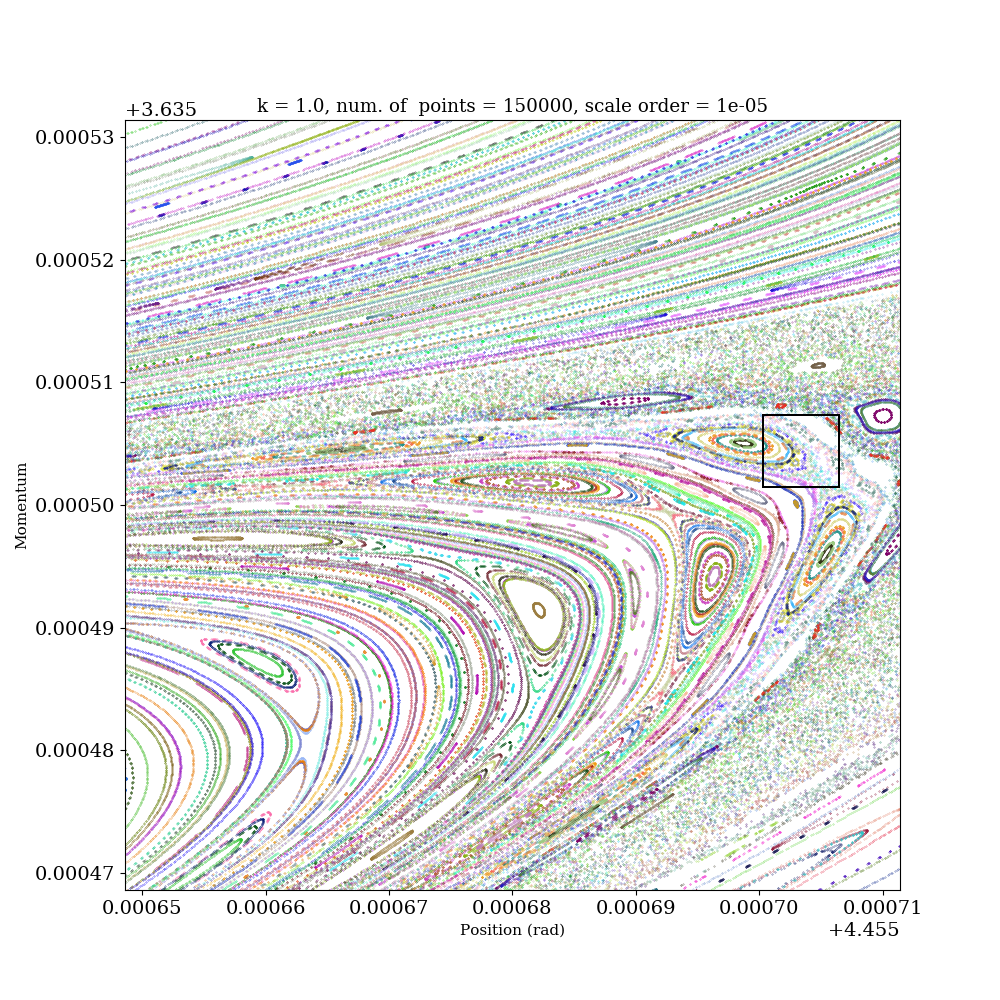
\includegraphics[width = 11cm]{stdmap6}
		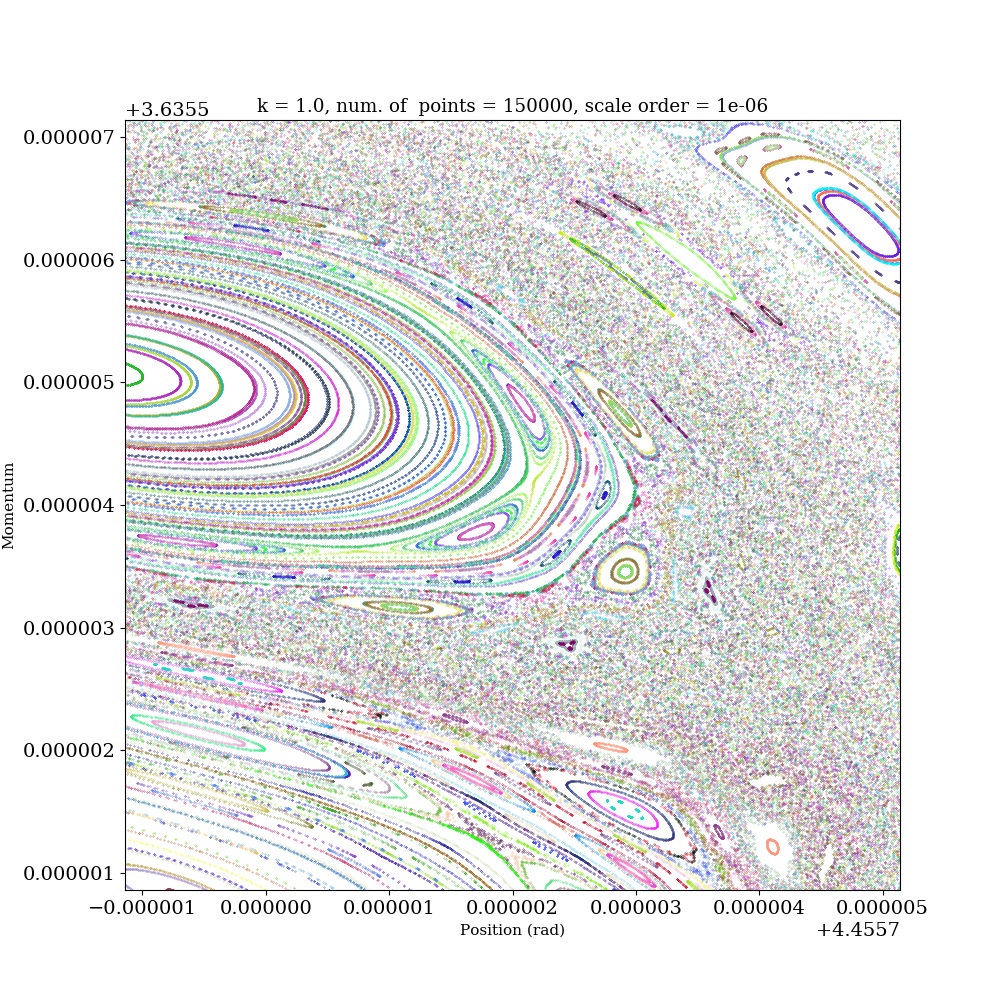
\includegraphics[width = 11cm]{stdmap7}
		\caption{Standardna preslikava pri k=1, enkratna (m=5) in dvokratna (m=6) pove"cava. Vir: \cite{1}}
		\label{slika 9}
	\end{center}
\end{figure}
\clearpage

\subsection{Rezultati}
Prepi"simo "se enkrat ena"cbo (\ref{1}) v 'angle-action' koordinatah ($I_1,\theta_1$) (identi"cen izraz)
\begin{equation}
\text{H}(I_1,\theta_1,t)=\frac{I_1^2}{2\bar{I}}+k\cos\theta_1\sum_n\delta(t-n\tau),\qquad \tau/\bar{I}=1.
\end{equation}
\begin{wrapfigure}[]{R}{0.5\textwidth}
	\begin{center}
		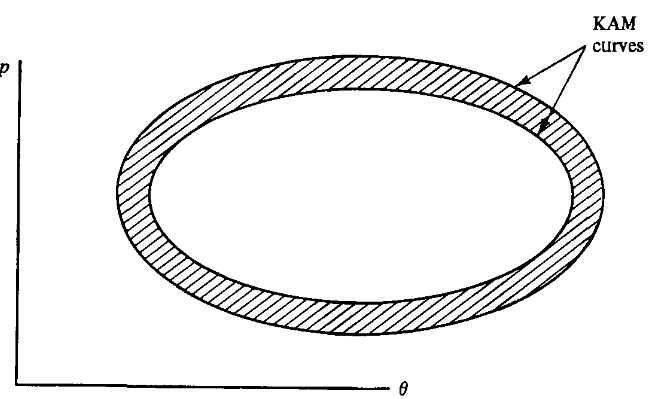
\includegraphics[width = 6cm]{9}
		\caption{Obmo"cje med dvema invariantnima KAM zankama se slika samo vase. Vir: \cite{1}}
		\label{slika 10}
	\end{center}
\end{wrapfigure}
Brcani rotor je Hamiltonski sistem z eno prostostno stopnjo (N=1), ki je periodi"cno odvisen od "casa s periodo $\tau$ (\ref{1}). Fazni prostor raz"sirimo na 2N+1=3, tako, da uvedemo novo kotno spremenljivk0 $\theta_2$, ki je sorazerna "casu, tako da velja
\begin{equation}
\theta_2+n\tau=\theta_2,\qquad n\in\mathbb{Z}-\{0\}.
\end{equation}

Na tak na"cin lahko prostovrte"ci rotator opazujemo na preseku torusa z ravnino $\theta_2=konst.$, velikost parametra $k$, ki je sorazmeren z intenziteto 'brcanja', pa obravnavamo kot perturbacijo "casovno neodvisnega dela Hamiltonijana.\newline Na slikah \ref{slika 6}-\ref{slika 9} je prikazana standardna preslikava pri razli"cnih pove"cavah. Na vsaki (razen zadnji) je ozna"ceno obmo"cje naslednje pove"cave. Slike so bile risane pri $k=1$, ki je zelo blizu kriti"cni vrednosti $k_c\approx0.971635406$, pri kateri razpade "se zadnji neresonantni torus, ki v $\theta_1$ te"ce "cez cel fazni prostor (od 0 do $2\pi$). Ta tako imenovani zlati krog (golden circle) izvira iz periodi"cne orbite z rotacijskim "stevilom $R$ enakim zlatemu rezu $(1+\sqrt{5}/2)$, ki je najbolj irracionalno (glede na (\ref{9}) najpo"casneje konvergira). V primeru Hamiltonskega sistema z eno prostostno stopnjo (N=1), katerega fazni prostor smo raz"sirili "se na "casovno dimenzijo, je namre"c $R$ neposredno vezan le na edino 'nepoljubno' ohranjeno koli"cino - energijo, ki dolo"ca frekvenco kro"zenja $\theta_1$ (seveda to velja pod pogojem $\tau/\bar{I}=1$, ki da diskretni ena"cbi (\ref{2}) brezdimenzijsko obliko ter obenem fiksira $\tau$, ki bi bil 'sorazmeren z $I_2$' v "casovno raz"sirjenem faznem prostoru).\newline
Razlog, da smo opazovali samopodobnost standardne preslikave prav v bli"zini $k_c$ je, da smo pri $k=k_c$ pri"ca neke vrste faznemu prehodu v smislu, da korelacijska dol"zina naraste preko vseh meja, kar pomeni, da je v tem obmu"cju $k$ Poincar\'jev fazni portret sebi-podoben preko razli"cnih velikostnih skal. Prav tako je $k_c$ meja, nad katero lahko moment $I_1$ neomejeno nara"s"ca. Difuzijo momenta pod $k_c$ prepoveduje Poincar\'e-Caratanov integralski teorem
\begin{equation}
\oint_{\Gamma_1}\big(\boldsymbol{p}d\boldsymbol{q}-Hdt\big)=\oint_{\Gamma_2}\big(\boldsymbol{p}d\boldsymbol{q}-Hdt\big),
\end{equation}
ki obenem tudi narekuje, da se bo obmo"cje med dvema invariantnima KAM zankama slikalo samo vase (slika \ref{slika 10}). \newline
Na slikah \ref{slika 6}-\ref{9} se lepo vidijo verige $\tilde{q}$ elipti"cnih otokov, ki imajo okoli sebe novih $\tilde{q}'$ elipti"cnih otokov, ki imajo spet okoli sebe $\tilde{q}''$ elipti"cnih otokov itd.
\clearpage
\begin{thebibliography}{9}
	\bibitem{1}
	Ott, E. (1993). {\it Chaos In Dynamical Systems}. Canada: Cambridge University Press
\end{thebibliography}

\end{document}